\documentclass[aspectratio=169]{beamer}

% ============================================================
% COMPLETE REFERENCE DECK -- everything, in detail.
% Not time-boxed; a master from which a short talk is cut.
% Visual style consistent with the 10-min deck.
% ============================================================

\usepackage{tikz}
\usepackage{amssymb}
\usepackage{booktabs}
\usepackage[T1]{fontenc}
\usepackage[utf8]{inputenc}
\usepackage{graphicx}
\usepackage{hyperref}
\usepackage{listings}
\usetikzlibrary{arrows.meta, positioning, calc, fit, backgrounds}

\usetheme{metropolis}
\metroset{numbering=fraction, progressbar=foot, block=fill, sectionpage=progressbar}

% ---- palette --------------------------------------------------------------
\definecolor{ink}{HTML}{20303A}
\definecolor{accent}{HTML}{2D9CDB}
\definecolor{accentdk}{HTML}{1B6FA8}
\definecolor{warm}{HTML}{E07A3F}
\definecolor{good}{HTML}{3DA35D}
\definecolor{faint}{HTML}{C9D3DA}
\definecolor{paper}{HTML}{FBFCFD}
\definecolor{codebg}{HTML}{F2F5F8}

\setbeamercolor{normal text}{fg=ink, bg=paper}
\setbeamercolor{frametitle}{fg=paper, bg=ink}
\setbeamercolor{alerted text}{fg=accentdk}
\setbeamercolor{progress bar}{fg=accent, bg=faint}
\setbeamerfont{frametitle}{size=\large}

\lstset{basicstyle=\ttfamily\scriptsize, breaklines=true, frame=single,
  backgroundcolor=\color{codebg}, rulecolor=\color{faint}, columns=fullflexible,
  keepspaces=true, xleftmargin=4pt, xrightmargin=4pt}

% ---- helpers --------------------------------------------------------------
\newcommand{\bignum}[2]{{\fontsize{30}{32}\selectfont\textbf{#1}}\\[2pt]{\footnotesize\color{ink!70}#2}}
\newcommand{\lab}[1]{{\footnotesize\color{ink!65}#1}}
\newcommand{\key}[1]{\textbf{\color{accentdk}#1}}

\title{Rotor in Rust}
\subtitle{Fast RISC-V machine-model generation, symbolic console
          arguments, differential validation, and a witness visualizer ---
          the complete account}
\author{Jasmin Begi\'{c} \quad$\cdot$\quad Daniel Wassie}
\institute{Advanced Systems Engineering --- University of Salzburg \\
           supervised by Christoph Kirsch}
\date{June 2026}

\begin{document}

{\setbeamercolor{background canvas}{bg=ink}\setbeamercolor{normal text}{fg=paper}
\begin{frame}\titlepage\end{frame}}

% ====================================================================
\begin{frame}{What this deck covers}
  \begin{columns}[T]
    \column{0.5\linewidth}
    \footnotesize
    \begin{enumerate}
      \item The problem and the pipeline
      \item Rotor in Rust --- architecture and fidelity
      \item Performance --- measured, not claimed
      \item Proving it in C --- the back-port
    \end{enumerate}
    \column{0.5\linewidth}
    \footnotesize
    \begin{enumerate}\setcounter{enumi}{4}
      \item Symbolic console arguments
      \item Differential validation (the equivalence campaign)
      \item The witness visualizer
      \item Conclusions and what we learned
    \end{enumerate}
  \end{columns}
  \vfill
  \begin{block}{One sentence}
    We rebuilt a RISC-V verification-model generator, made it
    $\sim$1000$\times$ faster, opened a new input surface, and ---
    crucially --- \alert{proved at every step that the new tool still tells
    the truth}.
  \end{block}
\end{frame}

% ####################################################################
\section{1. The Problem and the Pipeline}
% ####################################################################

\begin{frame}{Testing samples; verification proves}
  \begin{columns}[T]
    \column{0.54\linewidth}\footnotesize
      \textbf{Testing} --- \lab{run on chosen inputs, observe}
      \begin{itemize}\setlength\itemsep{0.15em}
        \item 8 bytes of input $= 2^{64}$ possibilities
        \item you try a handful; the crash can hide in the rest
        \item proves a program \emph{broke}, never that it is \emph{safe}
      \end{itemize}
      \vspace{0.3em}
      \textbf{Bounded model checking} --- \lab{all inputs at once, to depth $k$}
      \begin{itemize}\setlength\itemsep{0.15em}
        \item the unknown input is algebra, not a guess
        \item yes $\rightarrow$ a concrete witness input
        \item no $\rightarrow$ a guarantee up to $k$ steps
      \end{itemize}
    \column{0.42\linewidth}
      \centering\vspace{0.6em}
      {\fontsize{38}{40}\selectfont\textbf{$2^{64}$}}\\[3pt]\lab{inputs}\\[1em]
      {\Large vs.}\\[1em]
      {\fontsize{22}{24}\selectfont\textbf{1 question}}\\[2pt]\lab{for all of them}
  \end{columns}
\end{frame}

\begin{frame}{The pipeline}
  \centering\vspace{0.4em}
  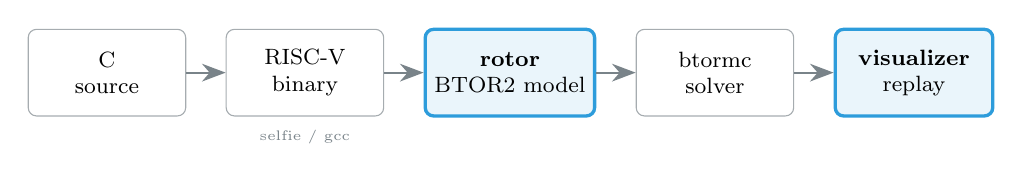
\begin{tikzpicture}[
      box/.style={draw=ink!40, rounded corners=3pt, minimum height=1.1cm,
                  minimum width=2.0cm, align=center, font=\footnotesize},
      ours/.style={box, draw=accent, fill=accent!10, very thick},
      arr/.style={-{Stealth[length=3mm]}, ink!60, thick}]
    \node[box]                       (src) {C\\source};
    \node[box, right=0.5cm of src]   (bin) {RISC-V\\binary};
    \node[ours, right=0.5cm of bin]  (mod) {\textbf{rotor}\\BTOR2 model};
    \node[box, right=0.5cm of mod]   (sol) {btormc\\solver};
    \node[ours, right=0.5cm of sol]  (vis) {\textbf{visualizer}\\replay};
    \draw[arr](src)--(bin);\draw[arr](bin)--(mod);\draw[arr](mod)--(sol);\draw[arr](sol)--(vis);
    \node[below=0.05cm of bin, font=\tiny, ink!60] {selfie / gcc};
  \end{tikzpicture}
  \vfill
  \begin{itemize}\setlength\itemsep{0.3em}
    \item \key{rotor} (part of selfie) translates a \emph{compiled binary}
          into a bit-precise model --- what is verified is what runs.
    \item \key{BTOR2} is the standard model format; \key{btormc} is the
          reference bounded model checker (Boolector project).
    \item The two highlighted stages are this project; selfie and btormc are
          unchanged third-party tools.
  \end{itemize}
\end{frame}

\begin{frame}{What a rotor model contains}
  A machine model is a board game: \key{state}, \key{rules},
  \key{forbidden positions}.
  \vspace{0.3em}
  \begin{columns}[T]
    \column{0.5\linewidth}
      \textbf{State} (one instant)
      \begin{itemize}\setlength\itemsep{0.15em}\footnotesize
        \item program counter, 32 registers
        \item memory arrays: code, data, heap, stack
        \item kernel: program break, file descriptor, input-buffer counters
      \end{itemize}
    \column{0.5\linewidth}
      \textbf{Rules + properties}
      \begin{itemize}\setlength\itemsep{0.15em}\footnotesize
        \item one transition function per state variable --- the semantics of
              every instruction in the binary
        \item 24 \key{bad-state} properties: the things that must never happen
      \end{itemize}
  \end{columns}
  \vspace{0.4em}
  \begin{block}{Machine input = uninitialized states}
    A BTOR2 state with no \texttt{init} may take any value initially, so the
    solver quantifies over it. This one device models stdin --- and later,
    \alert{console arguments}.
  \end{block}
\end{frame}

\begin{frame}[fragile]{A worked example: division-by-zero}
  The program reads one byte, subtracts 48, divides by the result. Input
  \texttt{'0'} (=48) makes the divisor zero.
  \begin{lstlisting}
[btor>mc] bad state property 7 reachable at bound k = 76 SATISFIABLE
  \end{lstlisting}
  \vspace{-0.3em}
  \begin{itemize}\setlength\itemsep{0.25em}\footnotesize
    \item \key{property 7} = division-by-zero; \key{k = 76} = the minimal
          number of machine steps from boot to the faulting instruction.
    \item Witness byte: \texttt{0x30 = '0'} --- found by logic, over all 256
          possible bytes.
    \item This pair --- \key{(property index, minimal bound $k$)} --- is the
          unit of comparison for the entire project.
  \end{itemize}
\end{frame}

% ####################################################################
\section{2. Rotor in Rust}
% ####################################################################

\begin{frame}{Why rebuild it}
  \begin{columns}[T]
    \column{0.5\linewidth}
      \textbf{The original \texttt{rotor.c}}
      \begin{itemize}\setlength\itemsep{0.25em}\footnotesize
        \item one file, $\sim$14{,}000 lines of C*
        \item hundreds of file-level globals
        \item per-core state in parallel arrays
        \item hard to read, extend, integrate
      \end{itemize}
    \column{0.5\linewidth}
      \textbf{The rewrite (Rust)}
      \begin{itemize}\setlength\itemsep{0.25em}\footnotesize
        \item modular crate, one file per concern
        \item typed node graph (\texttt{enum Op}), hash-consed
        \item explicit four-phase pipeline, no globals
        \item a clean base to \emph{extend}
      \end{itemize}
  \end{columns}
  \vfill
  \begin{block}{Same job}
    The rewrite emits the \alert{same 24 bad-state properties} as the
    reference --- same names, same order, same predicates, re-derived from
    \texttt{rotor.c}.
  \end{block}
\end{frame}

\begin{frame}{Architecture}
  \centering\footnotesize
  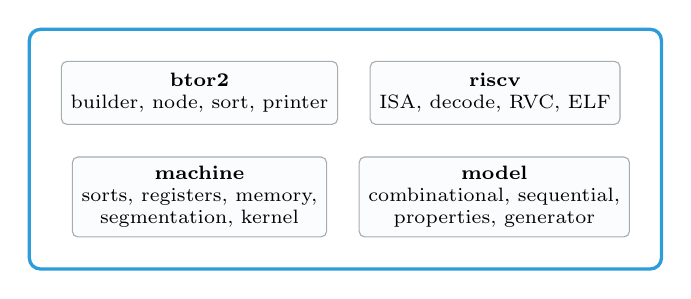
\begin{tikzpicture}[font=\scriptsize, node distance=2mm,
      m/.style={draw=ink!40, rounded corners=2pt, fill=paper, minimum width=2.6cm, minimum height=0.8cm, align=center}]
    \node[m] (b) {\textbf{btor2}\\ builder, node, sort, printer};
    \node[m, right=4mm of b] (r) {\textbf{riscv}\\ ISA, decode, RVC, ELF};
    \node[m, below=4mm of b] (mm) {\textbf{machine}\\ sorts, registers, memory,\\ segmentation, kernel};
    \node[m, right=4mm of mm] (mo) {\textbf{model}\\ combinational, sequential,\\ properties, generator};
    \begin{scope}[on background layer]
      \node[draw=accent, very thick, rounded corners=4pt, fit=(b)(r)(mm)(mo), inner sep=4mm] {};
    \end{scope}
  \end{tikzpicture}
  \vfill
  \begin{itemize}\setlength\itemsep{0.2em}\footnotesize
    \item Every BTOR2 node is a typed \texttt{enum Op}; structurally equal
          nodes are interned at creation through a hash map (Section 3).
    \item Four phases: load binary $\rightarrow$ build state $\rightarrow$
          generate logic + properties $\rightarrow$ print in topological order.
  \end{itemize}
\end{frame}

\begin{frame}{The 24 bad-state properties (emitted in this exact order)}
  \scriptsize
  \begin{columns}[T]
    \column{0.5\linewidth}
    \begin{tabular}{rl}
      b0 & illegal-instruction\\
      b1 & illegal-compressed-instruction\\
      b2 & known-instructions\\
      b3 & fetch-invalid-address\\
      b4 & fetch-unaligned\\
      b5 & fetch-seg-fault\\
      b6 & unknown-syscall-ID\\
      b7 & division-by-zero\\
      b8 & signed-division-overflow\\
      b9 & load-invalid-address\\
      b10 & store-invalid-address\\
      b11 & compressed-load-invalid-addr\\
    \end{tabular}
    \column{0.5\linewidth}
    \begin{tabular}{rl}
      b12 & compressed-store-invalid-addr\\
      b13 & stack-pointer-invalid-address\\
      b14 & load-seg-fault\\
      b15 & store-seg-fault\\
      b16 & compressed-load-seg-fault\\
      b17 & compressed-store-seg-fault\\
      b18 & stack-pointer-seg-fault\\
      b19 & brk-seg-fault\\
      b20 & openat-seg-fault\\
      b21 & read-seg-fault\\
      b22 & write-seg-fault\\
      b23 & bad-exit-code\\
    \end{tabular}
  \end{columns}
  \vspace{0.4em}
  \lab{Order matters: btormc identifies properties by index, so b7 means the
       same thing in both tools only if emission order matches.}
\end{frame}

\begin{frame}{Faithfulness: the modeled machine must be identical}
  Emitting the same properties is not enough --- the \emph{machine} feeding
  them must match, bit for bit. Differential validation forced each of these:
  \vspace{0.3em}
  \begin{itemize}\setlength\itemsep{0.3em}\footnotesize
    \item \key{Zeroed memory and registers} --- else the solver invents
          memory contents and produces spurious counterexamples.
    \item \key{Exact segment geometry} --- page-aligned heap, stack at
          $[\texttt{0xFFFFF800},\,2^{32})$ with the end wrapped to 0, program
          break at heap start; wrap-aware bounds checks.
    \item \key{Process-start stack image} --- concrete argc/argv layout, as
          selfie's boot loader writes it.
    \item \key{Read syscall} --- one input byte per machine transition, PC
          stalled while reading; exit stalls forever; file-descriptor state.
    \item \key{Property emission order} --- so indices line up.
  \end{itemize}
\end{frame}

\begin{frame}{The properties were ported, not guessed}
  Three of our first, plausible-looking property bodies were \emph{wrong} ---
  and the validation harness caught all three before they could mislead:
  \vspace{0.3em}
  \begin{itemize}\setlength\itemsep{0.35em}\footnotesize
    \item \key{brk validity}: we assumed a lower bound (new break $\geq$
          current). The reference checks only the upper bound, so
          \texttt{brk(0)} queries are valid --- our version fired a spurious
          fault at $k=5$.
    \item \key{openat}: we checked one address; the reference checks the
          range $[\mathit{a1}, \mathit{a1}+127]$ against the heap.
    \item \key{read-seg-fault}: we checked on every transition; the reference
          checks once, at the \emph{start} of the read.
  \end{itemize}
  \vspace{0.3em}
  \lab{None of these would have been caught by reviewing property names or
       comparing file sizes. Only the solver-level check exposed them.}
\end{frame}

% ####################################################################
\section{3. Performance --- Measured, Not Claimed}
% ####################################################################

\begin{frame}{The headline: three orders of magnitude}
  \centering\vspace{0.3em}
  Modeling selfie compiled to itself --- 43{,}406 RISC-U instructions.
  \vfill
  \begin{columns}[c]
    \column{0.5\linewidth}\centering
      \lab{GENERATION TIME}\\[6pt]
      {\large\color{warm}139\,s}\;{\large$\rightarrow$}\;\bignum{0.1\,s}{}
    \column{0.5\linewidth}\centering
      \lab{PEAK MEMORY}\\[6pt]
      {\large\color{warm}428\,MB}\;{\large$\rightarrow$}\;\bignum{20\,MB}{}
  \end{columns}
  \vfill
  \lab{Measured fairly: both consume the same pre-compiled binary, so
       compilation cost is excluded on both sides.}
\end{frame}

\begin{frame}{``Don't trust the number --- count.''}
  We instrumented the one operation both tools repeat millions of times:
  \emph{``is this subexpression already in the system?''}
  \vspace{0.2em}
  \centering\scriptsize
  \begin{tabular}{lrr}
    \toprule
     & C rotor & Rust rotor\\
    \midrule
    Node creations             & 3{,}171{,}632                  & 159{,}018\\
    Dedup question asked        & 9{,}976                        & 159{,}018\\
    Hits (already present)      & 6{,}021                        & 48{,}114\\
    \textbf{Basic operations}   & \textbf{\color{warm}11{,}695{,}232{,}963} & \textbf{\color{accent}159{,}018}\\
    Unique nodes in output      & 138{,}820                      & 110{,}904\\
    \bottomrule
  \end{tabular}
  \vspace{0.4em}\\
  \lab{Self-check: creations $-$ hits $=$ each tool's own reported line count,
       to the integer. A list walk (11.7 billion comparisons) vs.\ a hash
       probe (159k). That is the entire speed-up.}
\end{frame}

\begin{frame}{The cause, in one picture}
  \centering\vspace{0.3em}
  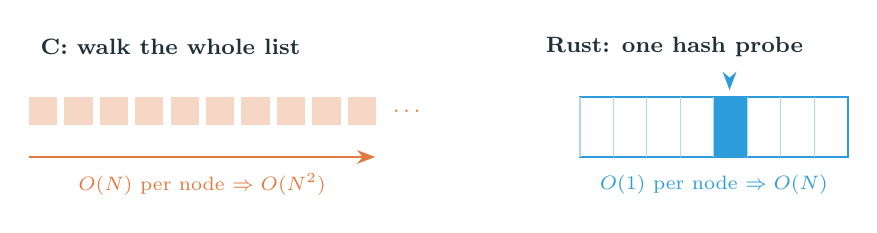
\begin{tikzpicture}[font=\footnotesize]
    % C: linear list
    \node[ink] at (-3.2, 2.4) {\textbf{C: walk the whole list}};
    \foreach \i in {0,...,9}{ \fill[warm!30] (-5+\i*0.45, 1.4) rectangle ++(0.36,0.36); }
    \node[warm] at (-0.2,1.58) {$\dots$};
    \draw[-{Stealth}, warm, thick] (-5.0,1.0) -- (-0.6,1.0);
    \node[warm, font=\scriptsize] at (-2.8,0.65) {$O(N)$ per node $\Rightarrow O(N^2)$};
    % Rust: hash
    \node[ink] at (3.2, 2.4) {\textbf{Rust: one hash probe}};
    \draw[accent, thick] (2.0,1.0) rectangle (5.4,1.76);
    \foreach \i in {0,...,7}{ \draw[accent!40] (2.0+\i*0.425,1.0) -- ++(0,0.76); }
    \fill[accent] (3.7,1.0) rectangle ++(0.425,0.76);
    \draw[-{Stealth}, accent, thick] (3.9,2.0) -- (3.9,1.85);
    \node[accent, font=\scriptsize] at (3.7,0.65) {$O(1)$ per node $\Rightarrow O(N)$};
  \end{tikzpicture}
  \vfill
  \lab{Same question, same answer, identical comparison logic. Only the data
       structure differs --- a list versus an index.}
\end{frame}

\begin{frame}{``Disable the duplicate check in both''}
  The supervisor's experiment, to rule out a hidden semantic difference:
  \vspace{0.3em}
  \begin{columns}[T]
    \column{0.5\linewidth}
      \textbf{C rotor, reuse off}
      \begin{itemize}\setlength\itemsep{0.2em}\footnotesize
        \item \alert{crashes} in 0.08\,s:\\ \texttt{ite then sort mismatch}
        \item it compares sorts by \emph{pointer}; reuse is what keeps the
              pointer-invariant true
        \item line reuse is load-bearing, not just speed
      \end{itemize}
    \column{0.5\linewidth}
      \textbf{Rust, \texttt{-{}-no-cse}}
      \begin{itemize}\setlength\itemsep{0.2em}\footnotesize
        \item runs fine; model grows $1.43\times$
        \item still well-formed; \emph{identical} solver verdict
        \item deduplication is provably cosmetic
      \end{itemize}
  \end{columns}
  \vfill
  \lab{Conclusion: deduplication affects size and speed, never meaning.}
\end{frame}

\begin{frame}{Why Rust beats even the optimized C}
  \centering\scriptsize
  \begin{tabular}{lrrr}
    \toprule
    selfie model & baseline C & C + hash & Rust\\
    \midrule
    Time          & 139\,s  & 1.5\,s  & $<$0.1\,s\\
    Memory        & 428\,MB & 485\,MB & 20\,MB\\
    Lines created & 3.17\,M & 3.17\,M & 159\,k\\
    \bottomrule
  \end{tabular}
  \vspace{0.5em}
  \begin{itemize}\setlength\itemsep{0.25em}\footnotesize
    \item The hash fixes the \key{lookup cost}. But C still \emph{creates}
          3.17M records and prunes later --- \key{create-then-filter}.
    \item Rust checks \emph{before} allocating; duplicates never exist ---
          \key{filter-at-creation}. That is the memory story and the last
          factor of speed.
  \end{itemize}
\end{frame}

\begin{frame}{Why the file sizes differ (same content, different spelling)}
  \centering\scriptsize
  \begin{tabular}{lrr}
    \toprule
    selfie model & with comments & comments stripped\\
    \midrule
    C rotor    & 10.59\,MB & 5.21\,MB \;\;(\textbf{50.8\%} was comments)\\
    Rust rotor & 3.12\,MB  & 2.97\,MB \;\;(5.0\%)\\
    \bottomrule
  \end{tabular}
  \vspace{0.5em}
  \begin{itemize}\setlength\itemsep{0.25em}\footnotesize
    \item Strip comments: the $3.4\times$ gap falls to $1.76\times$.
    \item The rest is encoding: C writes constants as 32/64-digit \emph{binary}
          strings, we write decimals; its node ids average 7 digits vs.\ our 5.
    \item Like pretty-printed-with-comments vs.\ minified JSON. Size is
          serialization; \alert{the solver establishes the meaning is identical}.
  \end{itemize}
\end{frame}

% ####################################################################
\section{4. Proving It in C --- The Back-Port}
% ####################################################################

\begin{frame}{The cleanest test of ``it is the data structure''}
  Make the change \emph{in the reference itself} --- hold the language fixed.
  \vspace{0.3em}
  \begin{itemize}\setlength\itemsep{0.3em}\footnotesize
    \item A $\sim$70-line patch to \texttt{tools/rotor.c}: replace the linear
          \texttt{find\_equal\_line} scan with an $O(1)$ hash-table probe over
          the same five identity fields, probing \emph{before} allocating.
    \item Two variants, both in C: a \key{byte-identical} one (keeps the
          reference's exact reuse decisions), and a \key{dedup-everywhere}
          one (mirrors the Rust rule).
  \end{itemize}
  \vfill
  \centering
  \begin{columns}[c]
    \column{0.33\linewidth}\centering\bignum{95$\times$}{faster, in the C}
    \column{0.33\linewidth}\centering\bignum{0}{output lines changed}
    \column{0.33\linewidth}\centering\bignum{36/36}{still equivalent}
  \end{columns}
\end{frame}

\begin{frame}{The back-port, in detail}
  \begin{itemize}\setlength\itemsep{0.3em}\footnotesize
    \item \key{Byte-identical variant}: selfie model in \textbf{1.5\,s} vs.\
          \textbf{139\,s} ($\sim$95$\times$); \texttt{diff} reports identical
          output on all 18 benchmarks and selfie (modulo the executable name
          in one header comment). Same source, compiler, output.
    \item \key{Dedup-everywhere variant}: a \emph{smaller} model (selfie:
          99k lines vs.\ baseline 139k), deduplicating every node except the
          kinds that must stay unique (state, input, init, next, bad,
          constraint, and the segment sorts). Passes the same \textbf{36/36}
          differential criterion (Section 6).
    \item \key{Bonus}: universal hash-consing makes the sort pointer-invariant
          hold everywhere, so the back-ported rotor \emph{no longer crashes}
          with reuse forced on --- realizing one of the fixes we proposed.
  \end{itemize}
\end{frame}

\begin{frame}{A failure worth keeping: naive ``dedup everything''}
  \begin{itemize}\setlength\itemsep{0.35em}\footnotesize
    \item A naive version --- deduplicate \emph{all} nodes, no exceptions ---
          yields a model where every benchmark reports a spurious bad state
          at \alert{bound 0}.
    \item Cause: the reference deliberately keeps its per-segment address and
          array sorts \emph{unique} (the regions guarded by
          \texttt{reuse\_lines = 0}). Merging them corrupts the initial state.
    \item So those regions are \key{correctness}, not just performance --- and
          the principled rule (keep those sorts unique) is what works.
  \end{itemize}
  \vfill
  \lab{The byte-identity check caught the naive version immediately; the
       differential criterion then certified the principled one. The method
       polices the optimization too.}
\end{frame}

% ####################################################################
\section{5. Symbolic Console Arguments}
% ####################################################################

\begin{frame}{A whole class of bugs was unreachable}
  \begin{columns}[c]
    \column{0.5\linewidth}\centering
      \lab{BEFORE}\\[6pt]
      {\large\ttfamily ./prog \textcolor{faint}{??????}}\\[6pt]
      {\footnotesize Command-line arguments were\\ \textbf{frozen} in the
       model.}
    \column{0.5\linewidth}\centering
      \lab{NOW}\\[6pt]
      {\large\ttfamily ./prog \textcolor{accent}{\textbf{??????}}}\\[6pt]
      {\footnotesize The solver fills the \textbf{open} bytes.}
  \end{columns}
  \vfill
  \begin{itemize}\setlength\itemsep{0.2em}\footnotesize
    \item The solver could only explore stdin; a bug needing \texttt{./prog
          SECRET} was structurally invisible --- not unfound, \emph{unlooked-for}.
    \item The original rotor paper lists ``console arguments as symbolic
          input'' as \alert{future work}. We built it.
  \end{itemize}
\end{frame}

\begin{frame}{Mechanism: the same device the paper already uses}
  \begin{itemize}\setlength\itemsep{0.3em}\footnotesize
    \item At process start the OS writes the argument strings, a pointer
          array, and \texttt{argc} onto the stack. We build exactly that
          layout.
    \item The \emph{content bytes} of \texttt{argv[1..N]} become
          \key{uninitialized one-byte states} --- the paper's own formal
          device for machine input. Everything else (\texttt{argc}, pointers,
          terminators, \texttt{argv[0]}) is concrete.
    \item The program reads them through \emph{ordinary} loads --- the decoder,
          memory model, and properties are untouched. The states are frozen
          (\texttt{next} = self), since arguments are fixed at exec time.
  \end{itemize}
  \vfill
  \lab{Soundness is inherited: a witness assignment is a real command line,
       and every command line within bounds is an admissible assignment.}
\end{frame}

\begin{frame}{The stack image at boot (symbolic mode)}
  \centering
  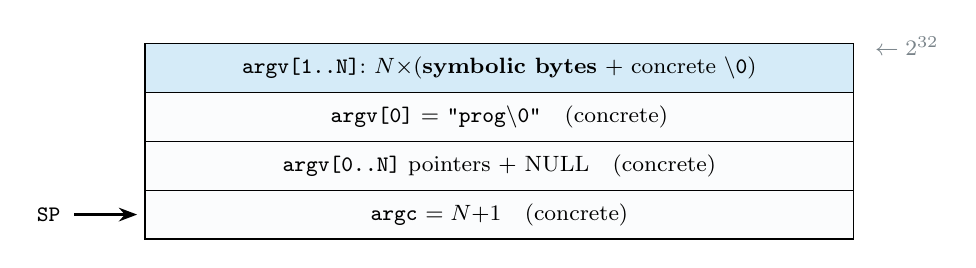
\begin{tikzpicture}[yscale=0.62, font=\footnotesize]
    \fill[accent!20](0,6)rectangle(9,7);\draw(0,6)rectangle(9,7);
    \node at(4.5,6.5){\texttt{argv[1..N]}: $N\times$(\textbf{symbolic bytes} + concrete \texttt{\textbackslash0})};
    \fill[paper](0,5)rectangle(9,6);\draw(0,5)rectangle(9,6);
    \node at(4.5,5.5){\texttt{argv[0]} = \texttt{"prog\textbackslash0"}\hspace{1em}(concrete)};
    \fill[paper](0,4)rectangle(9,5);\draw(0,4)rectangle(9,5);
    \node at(4.5,4.5){\texttt{argv[0..N]} pointers + NULL\hspace{1em}(concrete)};
    \fill[paper](0,3)rectangle(9,4);\draw(0,3)rectangle(9,4);
    \node at(4.5,3.5){\texttt{argc} $= N{+}1$\hspace{1em}(concrete)};
    \draw[-{Stealth},thick](-0.9,3.5)--(-0.1,3.5);\node[anchor=east]at(-0.95,3.5){\texttt{SP}};
    \node[anchor=west,ink!60]at(9.15,6.95){$\leftarrow 2^{32}$};
  \end{tikzpicture}
  \vfill
  \lab{Only the highlighted bytes are open (0--255); everything else is
       concrete, so the program's pointer chasing behaves exactly as on
       hardware.}
\end{frame}

\begin{frame}{Design choices (and their honest scope)}
  \begin{itemize}\setlength\itemsep{0.35em}\footnotesize
    \item \key{Argument count fixed} at generation time
          (\texttt{-{}-num-symbolic-args}); the solver explores \emph{content},
          not count --- symbolic count would need a dynamic layout.
    \item \key{Bounded length} (\texttt{-{}-max-arglen}), like the reference's
          bounded input buffer.
    \item \key{Interior zero bytes allowed} --- a shorter real-world string.
    \item \key{Fixed-slot layout} differs from packed \texttt{execve} only for
          programs that walk pointers past a terminator; for C-string programs
          the two are indistinguishable.
  \end{itemize}
  \vfill
  \lab{Where the paper is silent, these are our choices --- each keeps the
       model finite and static.}
\end{frame}

\begin{frame}{Five programs whose bugs live only in argv}
  None reads stdin, so none of these is reachable the old way.
  \vspace{0.2em}
  \centering\scriptsize
  \begin{tabular}{lll}
    \toprule
    Test & Bug fires when\dots & Class\\
    \midrule
    test1 & \texttt{argv[1][0] == 'C'} & one exact byte\\
    test2 & \texttt{argv[1][0]}$\cdot$256 + \texttt{argv[1][1]} $= 16706$ & ordered pair\\
    test3 & \texttt{argv[1][0]}$\neq 0 \wedge$ \texttt{argv[1][1]}$=0$ & a length property\\
    test4 & \texttt{argv[1][0]='X'} $\wedge$ \texttt{argv[2][0]='Y'} & two arguments\\
    test5 & \texttt{argv[1][0]} + \texttt{argv[1][1]} $= 200$ & arithmetic relation\\
    \bottomrule
  \end{tabular}
  \vspace{0.4em}
  \begin{block}{Verified (test1)}
    \footnotesize \texttt{bad-exit-code} SATISFIABLE at $k=67$, witness
    \texttt{argv[1][0] = 0x43 = 'C'} --- found through three pointer
    dereferences. All five solve within seconds.
  \end{block}
\end{frame}

\begin{frame}{The solver discovers the secret}
  \centering\vfill
  \colorbox{ink}{\color{paper}\large\ttfamily\;if (arg1[0]=='X' \&\& arg2[0]=='Y')\;\textcolor{warm}{crash}\;}
  \vfill
  {\large Two letters, in \alert{two different} arguments, at once.}\\[4pt]
  \lab{No keyboard input could ever trigger this.}
  \vfill
  {\large Solver, in seconds:\quad
   {\ttfamily arg1[0]=\textcolor{accent}{\textbf{X}}}\quad
   {\ttfamily arg2[0]=\textcolor{accent}{\textbf{Y}}}}
  \vfill
\end{frame}

% ####################################################################
\section{6. Differential Validation}
% ####################################################################

\begin{frame}{The criterion: let the solver be the referee}
  Textual comparison is meaningless (different spelling); formal equivalence
  is undecidable. Our checkable standard, in the spirit of differential
  testing:
  \vspace{0.3em}
  \begin{block}{}
    For the same binary and identical parameters, both models must make the
    \alert{same property index} satisfiable at the \alert{same minimal bound
    $k$} --- or both remain unsatisfiable to the limit.
  \end{block}
  \vspace{0.3em}
  \begin{itemize}\setlength\itemsep{0.2em}\footnotesize
    \item $k$ counts every transition from boot to the violation --- a
          fingerprint of the whole run; one wrong instruction shifts it.
    \item The verdict quantifies over all inputs, so no difference can hide
          behind input choice.
  \end{itemize}
\end{frame}

\begin{frame}{Setup}
  \begin{itemize}\setlength\itemsep{0.3em}\footnotesize
    \item The same 18 C* programs as the rotor paper
          (\texttt{examples/symbolic}), each with one input byte; same machine
          configuration (64-bit words, 32-bit address space, 2048-byte
          heap/stack).
    \item Reference models generated by the \emph{unmodified} C rotor (the
          command is recorded in each output file's header); our models with
          matching parameters.
    \item Validate both with \key{catbtor} (well-formedness) and a $k{=}0$
          \key{btormc} load, then run \texttt{btormc} to $k_{\max}=1500$ ---
          covering the paper's reported 66--1438 bug range.
    \item Each (benchmark, rotor) pair is an isolated container, parallelised
          across cores.
  \end{itemize}
\end{frame}

\begin{frame}{Results, configuration 1 (target exit code 0)}
  \centering\scriptsize
  \begin{tabular}{lll}
    \toprule
    Benchmark & Property (both) & $k$\\
    \midrule
    division-by-zero & division-by-zero & 76\\
    invalid-memory-access-fail & store-invalid-address & 79\\
    memory-access-fail & load-seg-fault & 66\\
    recursive-ackermann & bad-exit-code & 152\\
    recursive-factorial-fail & bad-exit-code & 119\\
    recursive-fibonacci & bad-exit-code & 118\\
    nested-if-else / -reverse & bad-exit-code & 100 / 103\\
    simple-* (6 programs) & bad-exit-code & 91--108\\
    three-/two-level-nested-loop & bad-exit-code & 103 / 99\\
    nested-recursion-fail, return-from-loop & --- & UNSAT@1500\\
    \bottomrule
  \end{tabular}
  \vspace{0.4em}\\
  \lab{16 satisfiable rows (5 distinct property types), 2 agreed-UNSAT ---
       \textbf{18/18} identical. Lowest bound 66 = the paper's lowest.}
\end{frame}

\begin{frame}{Results, configuration 2 (target exit code 1) --- and a flip}
  Re-run with both rotors targeting exit code 1 (the paper's planted
  ``non-zero exit'' bugs). \alert{18/18 again.}
  \vspace{0.3em}
  \begin{itemize}\setlength\itemsep{0.25em}\footnotesize
    \item The three exit-independent properties fire at unchanged bounds.
    \item Five planted bugs fire at $k \in [91,107]$ with identical $k$.
    \item \key{return-from-loop} \emph{flips}: UNSAT under target 0, SAT at
          $k=95$ under target 1 --- and \emph{both rotors flip identically}.
  \end{itemize}
  \vfill
  \begin{block}{Total}
    \textbf{36 paired verdicts across two configurations, zero divergences.}
    The agreement survives parameter change --- it is not an artifact of one
    setting.
  \end{block}
\end{frame}

\begin{frame}{The criterion at work: it failed loudly, on purpose}
  Every modeling defect we introduced was caught \emph{here} first:
  \vspace{0.3em}
  \centering\scriptsize
  \begin{tabular}{ll}
    \toprule
    Defect during development & How the check exposed it\\
    \midrule
    uninitialized segment arrays & wrong property at a shallow bound\\
    missing argv boot image & division benchmark became a read fault\\
    mis-ported brk predicate & spurious fault at $k=5$\\
    \bottomrule
  \end{tabular}
  \vspace{0.5em}\\
  \lab{The final all-green table was reached by fixing \emph{models}, never by
       weakening the criterion. A criterion that detected every defect on the
       way is one whose final ``pass'' carries weight.}
\end{frame}

\begin{frame}{The harness caught \emph{itself}}
  \begin{itemize}\setlength\itemsep{0.3em}\footnotesize
    \item In the parallel run, three benchmarks first showed
          \key{DIVERGE} --- but a baseline reported UNSAT where the reference
          fires \texttt{bad-exit-code}, which is impossible.
    \item Cause: under memory pressure a \texttt{btormc} container was killed,
          and its empty output was misread as UNSAT.
    \item Re-run \emph{sequentially}: all three match exactly
          (\texttt{bad-exit-code} @ 100, 119, 103). The runner now
          distinguishes ``completed, nothing reachable'' from ``no output''.
  \end{itemize}
  \vfill
  \lab{We caught it because one row disagreed with the other seventeen ---
       an anomaly against the reference triggers investigation, not
       acceptance. The methodology polices itself.}
\end{frame}

\begin{frame}{What we do \emph{not} claim}
  \begin{itemize}\setlength\itemsep{0.35em}\footnotesize
    \item Not a formal proof of generator equivalence --- that is undecidable,
          and the paper's own future work.
    \item Evidence is bounded: 18 programs, depth 1500, two configurations.
    \item Two benchmarks agree only by \emph{both} finding nothing (UNSAT) ---
          weaker than a step-exact match.
    \item Paths the suite does not exercise (compressed-instruction execution,
          gcc's W-suffixed arithmetic) are ported but not differentially
          validated.
  \end{itemize}
  \vfill
  \lab{The strength of the claim is that it is falsifiable --- and it
       \emph{was} falsified, repeatedly, until it was not.}
\end{frame}

% ####################################################################
\section{7. The Witness Visualizer}
% ####################################################################

\begin{frame}[fragile]{The problem: the answer is unreadable}
  What \texttt{btormc} returns when it finds a bug:
  \begin{lstlisting}
sat
b23
#0
3 01000011 argv[1][0]#0
4 10000010 argv[1][1]#0
; ... thousands of lines keyed to internal node numbers ...
  \end{lstlisting}
  \vspace{-0.2em}
  \lab{Sound, complete --- and humanly opaque. A correct answer nobody can
       read convinces nobody.}
\end{frame}

\begin{frame}{The model, made readable}
  \vfill
  \begin{columns}[c]
    \column{0.46\linewidth}\centering
      \fbox{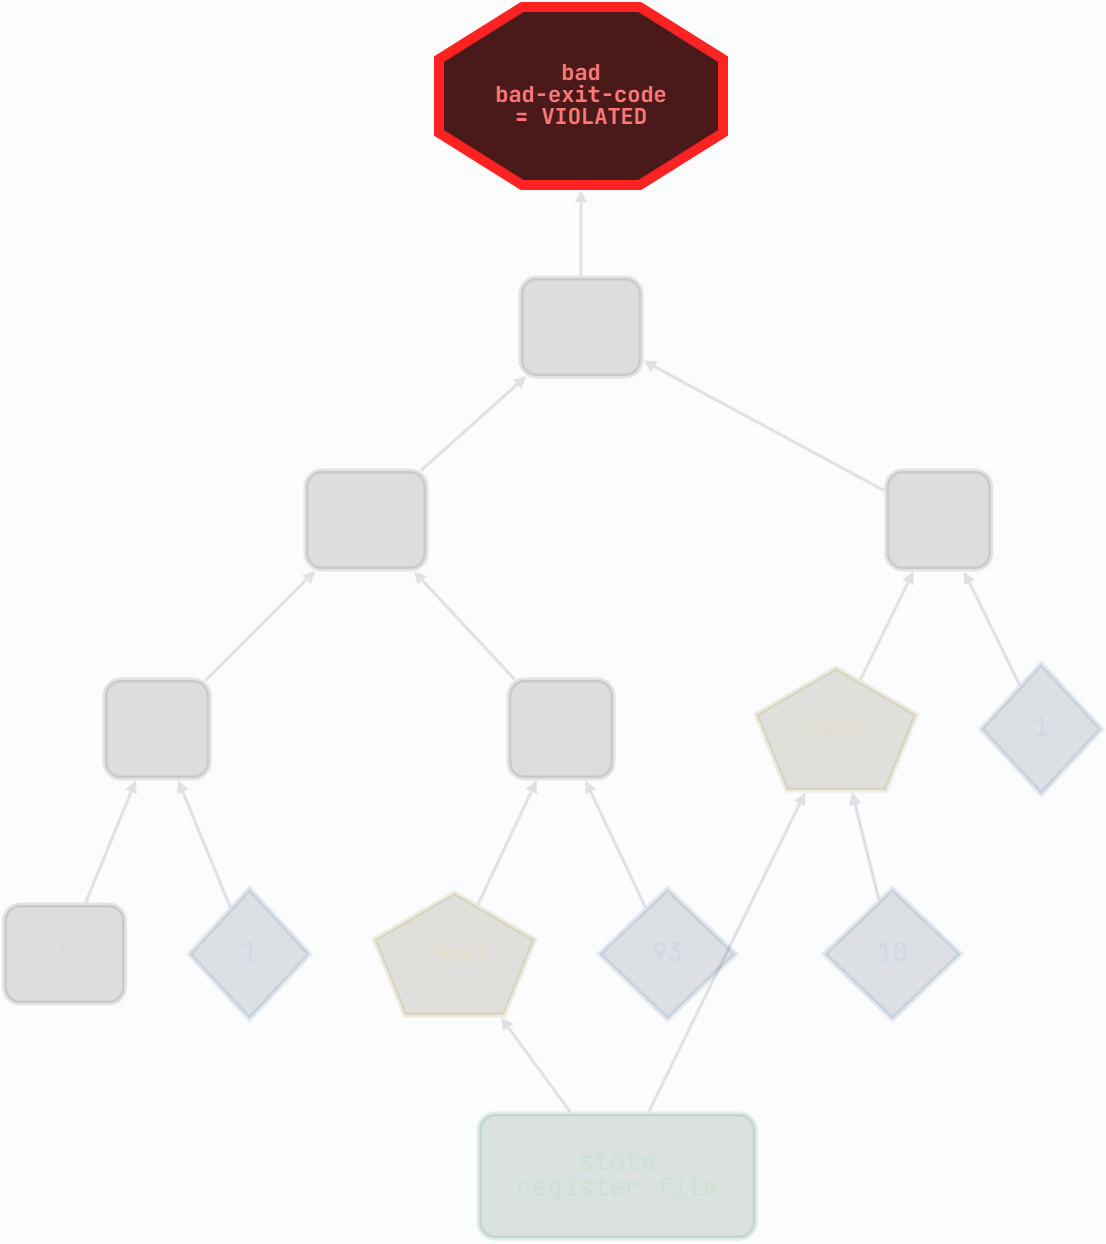
\includegraphics[height=0.66\textheight]{figures/visualizer_graph.png}}
    \column{0.5\linewidth}\footnotesize
      The model as an interactive graph; the witness replayed on top.
      \begin{itemize}\setlength\itemsep{0.2em}
        \item nodes shaped/coloured by role --- the red octagon is the bad
              state, \textcolor{warm}{\textbf{bad-exit-code VIOLATED}}
        \item cone-of-influence views, depth limits, collapsing, clumping,
              search, PNG/SVG export
        \item timeline scrubber, keyboard shortcuts, drag \& drop; 12 examples
              preloaded
      \end{itemize}
      \lab{Online, no install: jaspek.github.io/rotor-rust}
  \end{columns}
  \vfill
\end{frame}

% ####################################################################
\section{8. Conclusions}
% ####################################################################

\begin{frame}{What we delivered}
  \begin{itemize}\setlength\itemsep{0.4em}\footnotesize
    \item \key{Rotor in Rust} --- modular, $\sim$1000$\times$ faster
          generation, $21\times$ less memory, same 24 checks; behaviour
          verified per benchmark by an independent solver.
    \item \key{Symbolic console arguments} --- the paper's named future-work
          item, built with the paper's own formal device; five argv-only bugs
          found in seconds.
    \item \key{A differential-validation methodology} --- 36/36 paired
          verdicts; it caught every defect, one crash in the reference, and
          one bug in our own harness.
    \item \key{A back-port to C} --- the optimization in the reference itself:
          $\sim$95$\times$, byte-identical, 36/36. The cause is the data
          structure, not the language.
    \item \key{A witness visualizer} --- the answer as a readable, replayable
          graph; online.
  \end{itemize}
\end{frame}

\begin{frame}{What we learned}
  \vfill
  \centering
  {\large The hard part of rebuilding a verification tool is not\\
   writing the code.}\\[0.6em]
  {\large It is \alert{proving the new one still tells the truth}.}
  \vfill
  \lab{Speed was one data structure. Trust was the whole project --- and the
       methodology that delivered it (count, compare, let the solver judge,
       investigate every anomaly) is the part that transfers to the next
       tool.}
  \vfill
\end{frame}

\begin{frame}{Future work}
  \begin{itemize}\setlength\itemsep{0.35em}\footnotesize
    \item Symbolic argument \emph{count} and packed \texttt{execve} string
          layouts.
    \item Symbolic environment variables and file contents (needs
          file-descriptor modeling).
    \item Extend differential validation to gcc binaries exercising the
          compressed and W-suffixed instruction paths.
    \item Deeper bounds for the two agreed-UNSAT benchmarks; the selfie
          self-model at depth.
    \item Semantic deduplication (commutativity, identities) beyond the
          syntactic check.
    \item As for the reference --- formal verification of the generator
          itself.
  \end{itemize}
\end{frame}

\begin{frame}[standout]
  Thank you.\\[0.6em]
  {\small github.com/jaspek/rotor-rust \;$\cdot$\;
   github.com/jaspek/rotor-c-hashcons \;$\cdot$\;
   jaspek.github.io/rotor-rust}
\end{frame}

\end{document}
